\chapter{РАЗРАБОТКА ПРОГРАММНОГО ИНТЕРФЕЙСА}

Сначала в данной главе будет произведен поверхностный обзор интерфейса прикладного программирования робота. Подробно рассматриваться данный компонент не будет в связи с тем, что все управление роботом в дальнейшем будет производиться через методы классов, предоставляемых симулятором Webots. Взаимодействие с интерфейсом DARwIn Framework будет происходить только при компиляции модуля для интерпретации непоследственно на самом роботе. Это связано с тем, что вызовы методов классов Webots для управления моторами на физической модели робота имеют существенные задержки во времени, которые не позволяют роботу совершать плавные и непрерывные движения.

Так же кратко будет рассмотрен интерфейс управления приводами одного из самых распространенных гуманоидных роботов Nao. Этот анализ будет произведен для получения представления о имеющихся аналогах систем управления: их плюсах и недостатках.

Далее, исходя из ранее полученных знаний, будет разработан интерфейс класса для языка программирования C++. Другие популярные языки высокого, такие как Java и Python, были исключены из-за их низкой производительности. Для поддержки данных языков в реализованного модуля управления можно воспользоваться инструментом связывания программ и библиотек, написанных на языке C и C++, с интерпретируемыми (Tcl, Perl, Python, Ruby, PHP) или компилируемыми (Java, C\#, Scheme, OCaml) языками - SWIG.


\section{Обзор DARwIn Framework}

В данном разделе будет произведет поверхностный обзор системы управления роботом, предоставляемого разработчиками платформы.

Исходный код фреймфорка, написанного на языке C/C++, для платформы DARwIn-OP можно получить из репозитория проекта на сайте SourceForge. Исходный код распространяется под открытой лицензией. Так же используемые в данной работе классы доступны в пакете симуляции Webots в каталоге с модулями для данного робота. Симуляционная среда будет подробнее рассматриваться в следующем разделе.

Ниже приведена диаграмма классов (Рис. \ref{im:1_framework_class_diagram}), доступная в официальной документации. На данной диаграмме отображены все основные классы, которые используются при взаимодействии с роботом. % TODO Ссылка на документацию

\begin{figure}[h]
\center{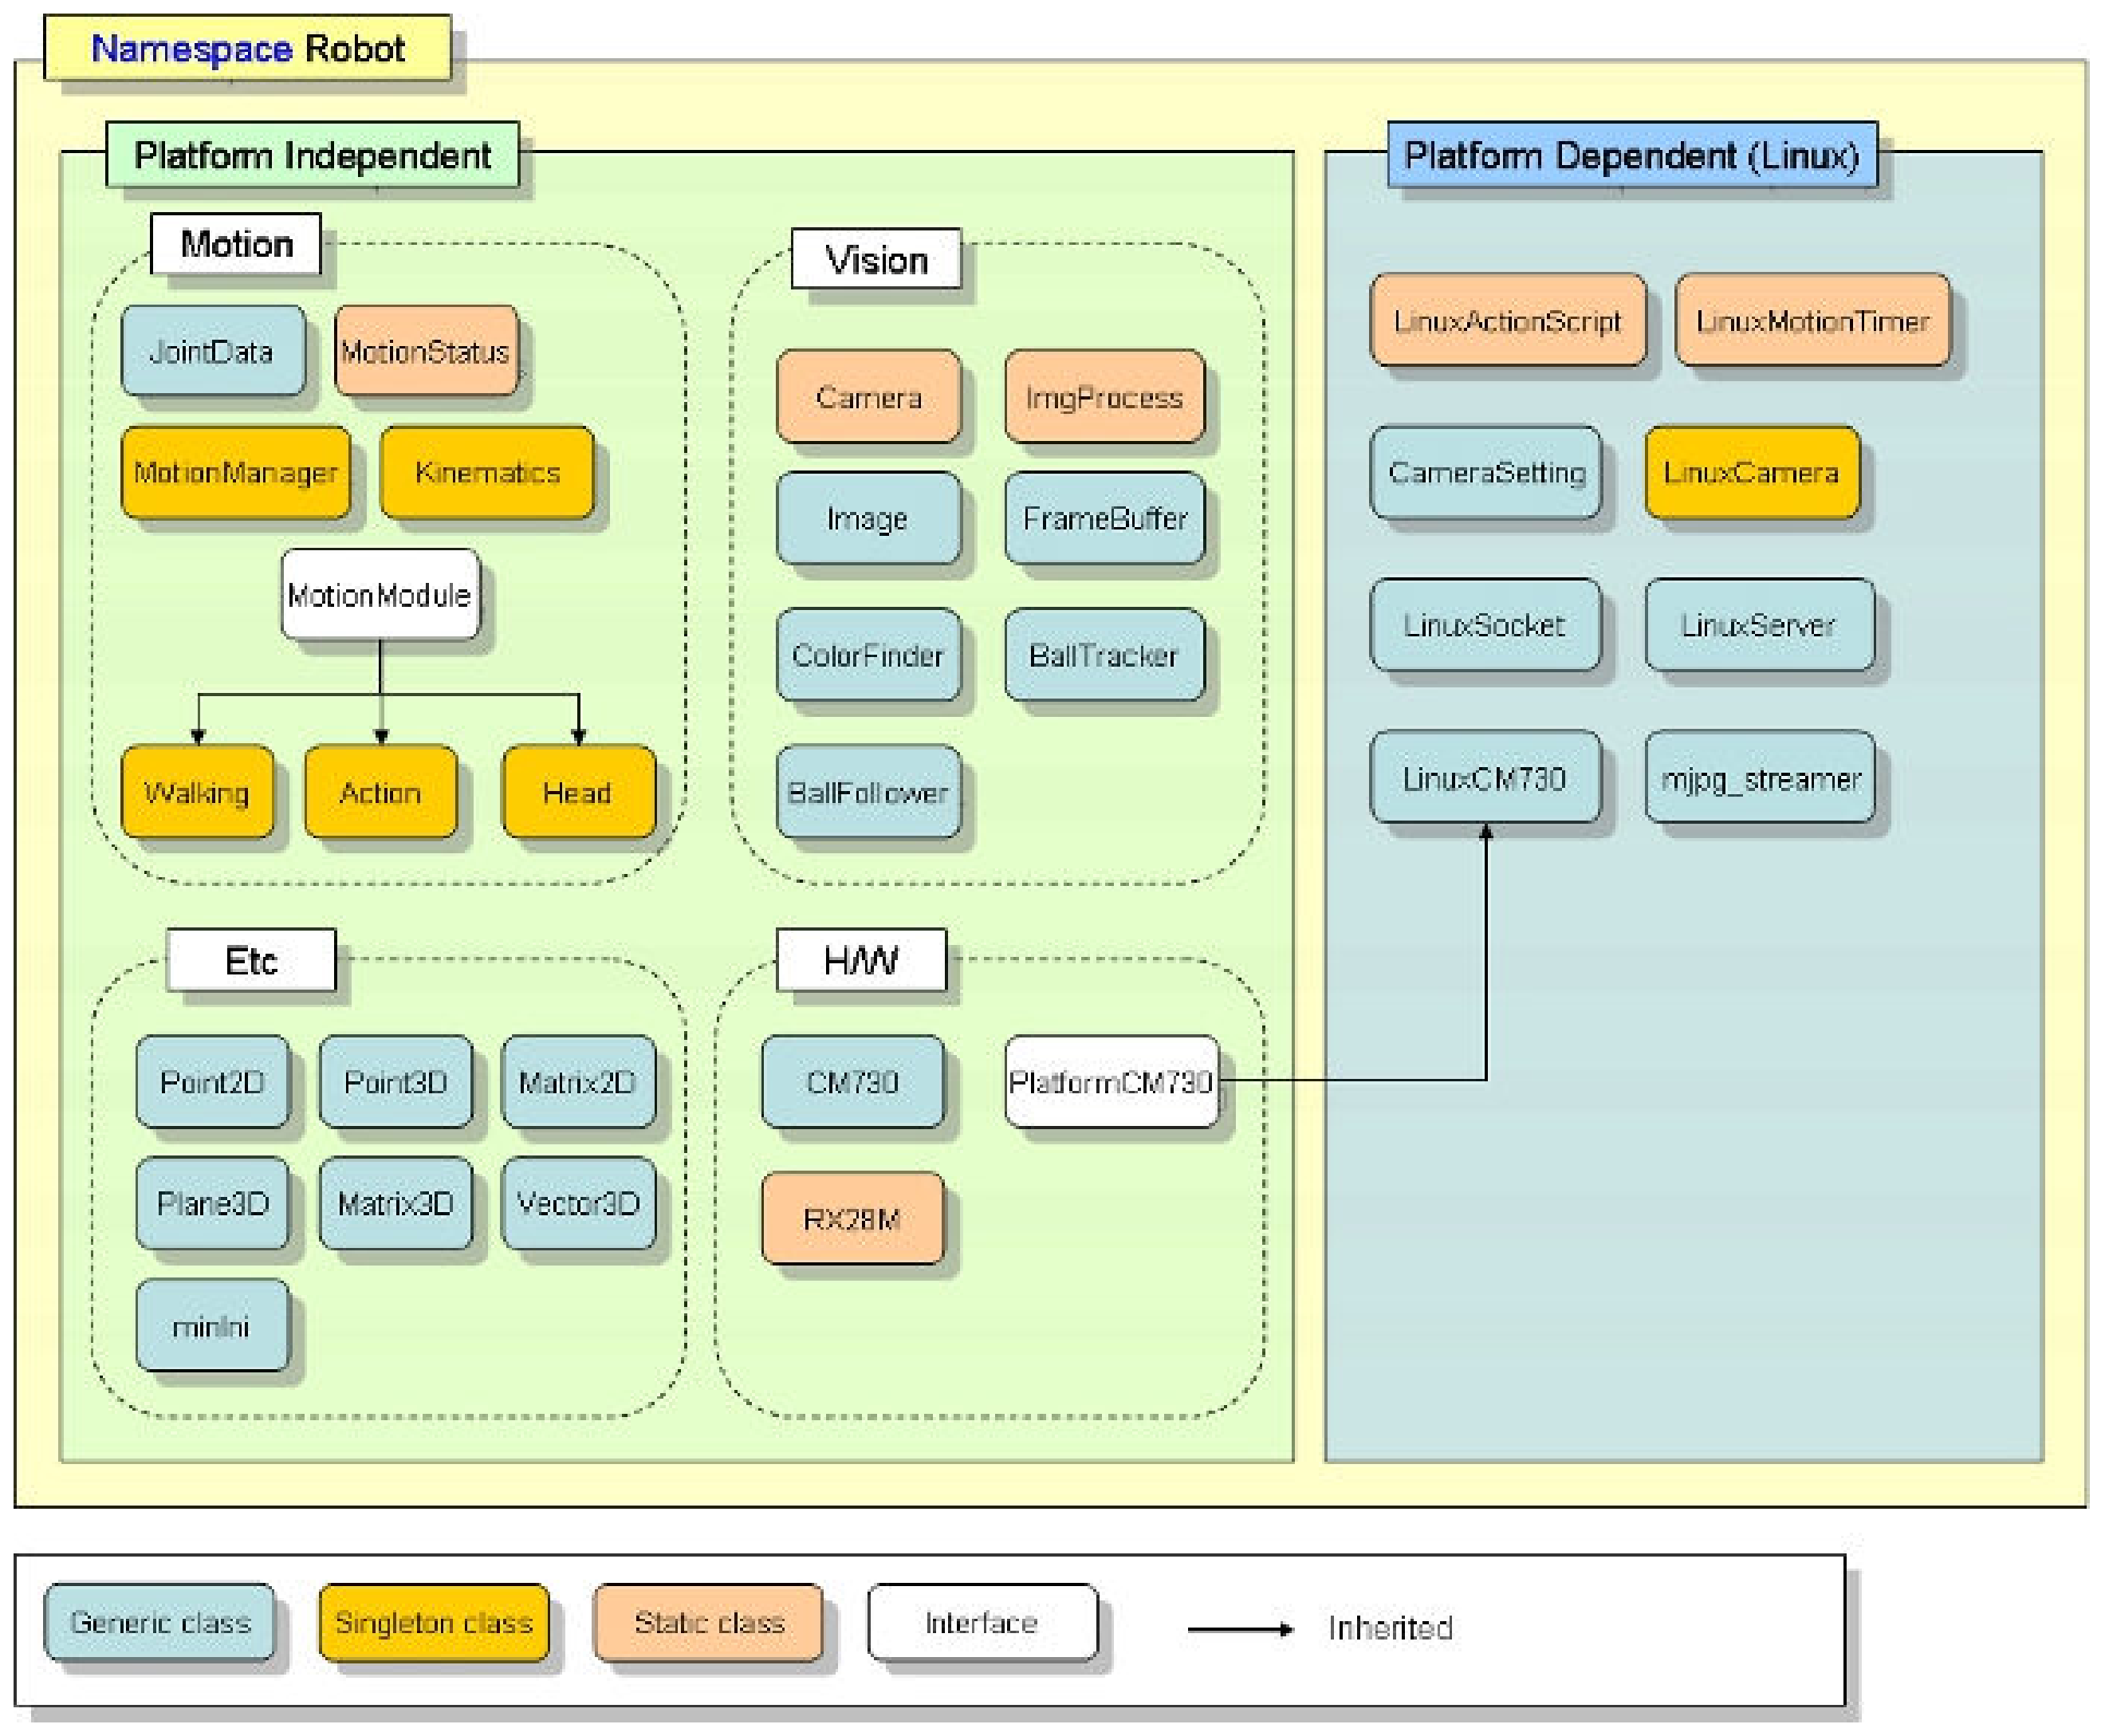
\includegraphics[width=1\linewidth]{1_framework_class_diagram}}
\caption{Диаграмма классов DARwIn Framework.}
\label{im:1_framework_class_diagram}
\end{figure}

Все классы находятся в области видимости Robot и делятся на платформонезависимые элементы и элементы, написанные для операционной системы Linux. Сам робот работает под управлением операционной системы Linux Ubuntu 9.10. Из данных классов нас будут интересовать елементы групп H/W и Motion.

Класс CM730 отвечает за взаимодействие программы-контроллера с субконтроллером робота. Он предоставляет возможность получать информацию с устройств, подключенных к данной плате (гироскоп, акселерометр, кнопки, сервоприводы и т.д.), а так же отправлять данные на светодиодные индикаторы и сервоприводы. Отправка и получение данных с соответствующих устройств происходит с задержкой в 6 мс. Для увеличения производительности отправка и получение данных на все моторы робота происходит единым пакетом данных.

Для управления движениями робота была реализованна группа классов Motion. Класс JointData является контейнером данных для взаимодействия с моторами робота. Он хранит PID данные и позиции для каждого сервопривода, а так же предоставляет публичные методы для взаимодействия с этими переменными.

Класс Kinematics имеет статические поля с информацией о длинах состовляющих ноги робота (высота бедра, голени и стопы) и информация о позиции камеры. Информации о длинах состовляющих рук в данном классе отсутствуют и дальнейшем будут взяты из документации о кинематике робота. % TODO Ссылка на документацию

MotionModule является интерфейсом для управления движениями робота. Данный интерфейс хранит экземпляр JointData для взаимодействия алгоритма с моторами. Производитель робота предоставляет в данном фреймворке готовый модуль управления походкой робота (Walking), модуль вопроизведения записанных движений (Action) и модуль для управления головой робота (Head).

Подробнее стоит рассмотреть реализацию модуля походки робота. Параметры походки читаются из конфигурационного *.ini файла с помощью библиотеки miniIni, которая идет в комплекте с данным фреймворком. Далее приведены основные параметры, которые описываются в файле: начальное смещение стопы по оси X в миллиметрах, начальное смещение стопы по оси Y в миллиметрах, начальное смещение стопы по оси Z в миллиметрах, начальный разворот стопы стопы вокруг оси X в градусах, начальный разворот стопы стопы вокруг оси Y в градусах, начальный разворот стопы стопы вокруг оси Z в градусах, угол наклона туловища в градусах, период двух шагов в миллисекундах, соотношение времени между периодом переноса ноги и остановки, длина шага в миллиметрах, максимальная амплитуда поднятия стопы в миллиметрах, амплитуда смещения туловища влево-вправо в миллиметрах, амплитуда подъема-опускания туловища в миллиметрах. Данный перечень параметров можно сгруппировать в параметры положения и вращения туловища и параметры положения и вращения левой и правой стопы, что пригодится в дальнейшем при разработке системы управления роботом. Сам алгоритм походки состоит и поочередного переноса стопы по синусоидальной траектории: высчитывается позиция стопы в каждый момент времени и решается задача обратной кинематики для расчета позиций моторов. Так же стоит обратить внимание, что алгоритм реализован некорректно при развороте стопы вокруг оси Z и ненулевом наклоне туловища: наклон робота происходит путем добавления угла наклона к позиции моторов бедер, а при вращении ноги вокруг оси Z данный угол должен был распределяться на два мотора на каждой ноге. В разработке системы управления механикой этот фактор так же будет учтен.

Статический класс MotionStatus является контейнером для данных, полученных с гироскопа, акселерометра и кнопок робота.

Класс MotionManager является связующим звеном между реализациями MotionModule и MotionStatus с классом CM730: класс передает данные из активных модулей движения непосредственно на физические моторы.
Для демонстрации взаимодействия классов ниже приведена схема передачи данных между модулями робота (Рис. \ref{im:1_framework_pipeline}), приведенная в официальной документации робота.

\begin{figure}[h]
\center{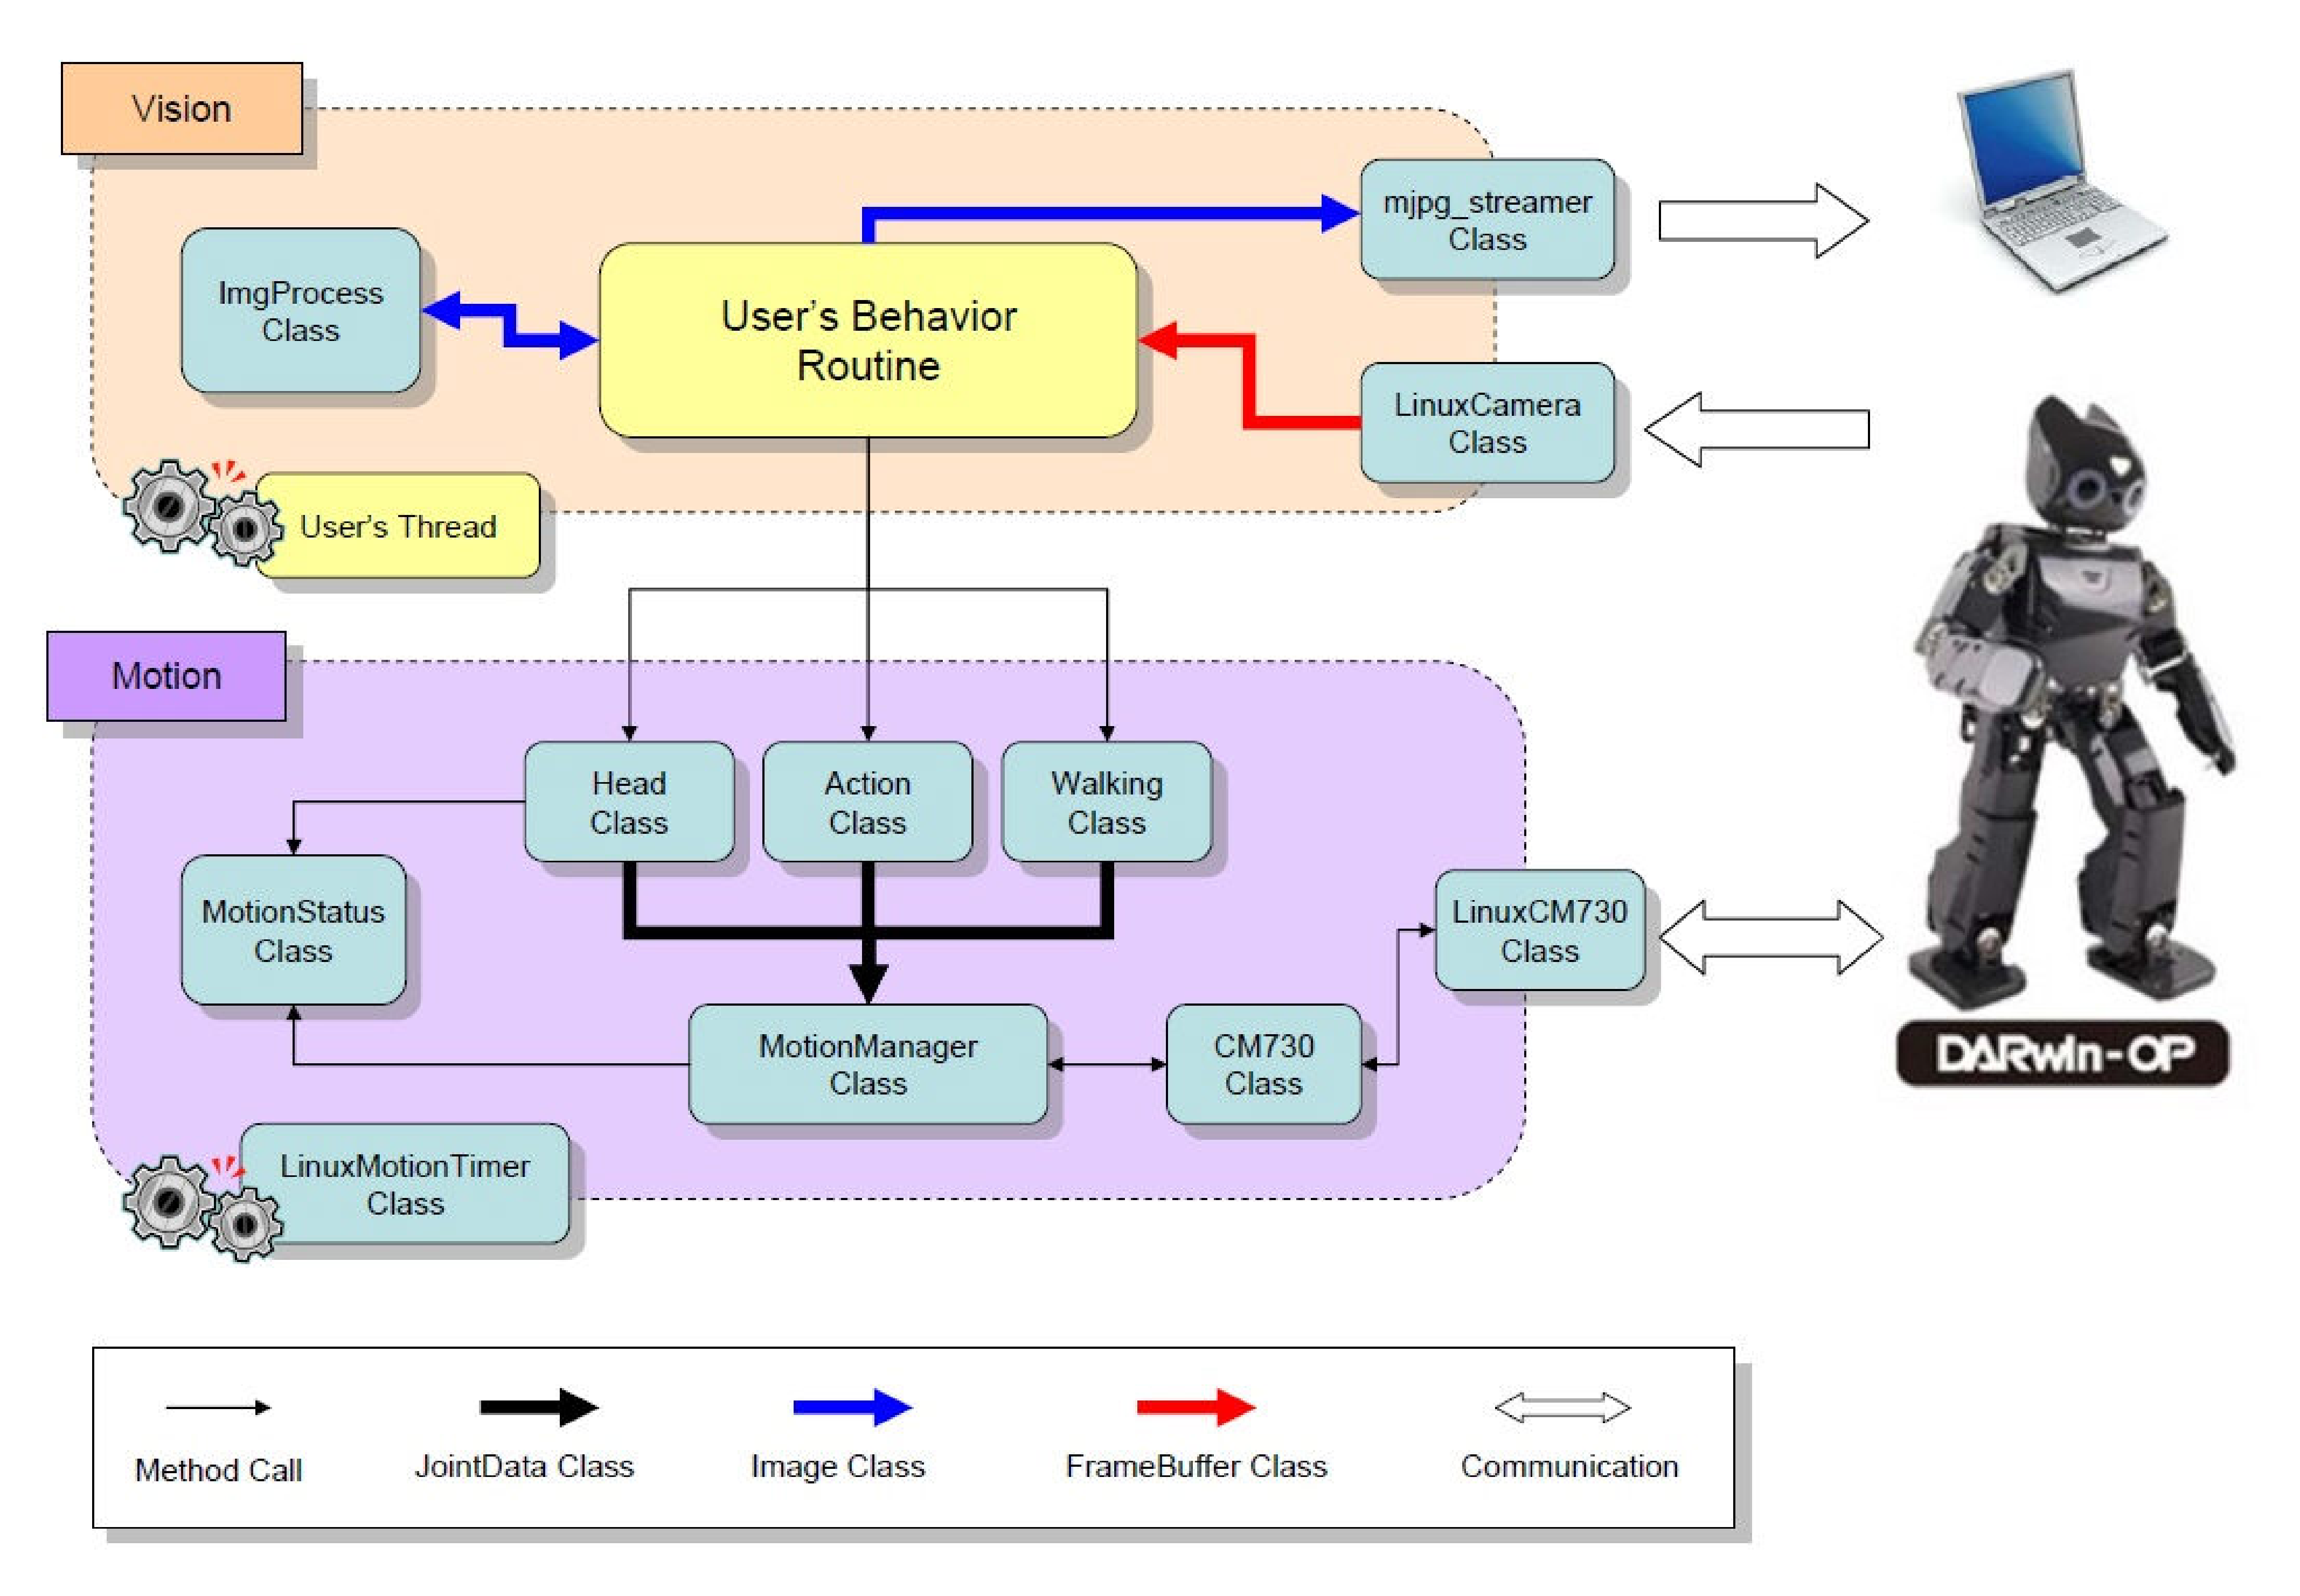
\includegraphics[width=1\linewidth]{1_framework_pipeline}}
\caption{Диаграмма передачи данных между модулями робота.}
\label{im:1_framework_pipeline}
\end{figure}

Обобщив выше сказанное можно заметить, что в интерфейсе программирования роботом отсутствует готовая реализация механизма программным управлением движений с помощью перемещений декартовой системы координат. Исходя из этого можно утверждать, что, например, при игре в футбол возможности удара по мячу у данного робота ограничивается механизмом воспроизведения записанных движений и отсутствует возможность расчета траектории удара. 
